%\documentclass[wcp,gray]{jmlr} % test grayscale version
\documentclass[wcp]{jmlr}

% The following packages will be automatically loaded:
% amsmath, amssymb, natbib, graphicx, url, algorithm2e

%\usepackage{rotating}% for sideways figures and tables
\usepackage{longtable}% for long tables

% The booktabs package is used by this sample document
% (it provides \toprule, \midrule and \bottomrule).
% Remove the next line if you don't require it.
\usepackage{booktabs}
% The siunitx package is used by this sample document
% to align numbers in a column by their decimal point.
% Remove the next line if you don't require it.
%\usepackage[load-configurations=version-1]{siunitx} % newer version
%\usepackage{siunitx}

% The following command is just for this sample document:
\newcommand{\cs}[1]{\texttt{\char`\\#1}}

\jmlrvolume{XX}
\jmlryear{2016}
\jmlrworkshop{BIGMINE 2016}

\title[Scalable SDE Filtering and Inference]{Scalable SDE Filtering and Inference with Apache Spark}

 % Use \Name{Author Name} to specify the name.
 % If the surname contains spaces, enclose the surname
 % in braces, e.g. \Name{John {Smith Jones}} similarly
 % if the name has a "von" part, e.g \Name{Jane {de Winter}}.
 % If the first letter in the forenames is a diacritic
 % enclose the diacritic in braces, e.g. \Name{{\'E}louise Smith}

 % Two authors with the same address
 % \author{\Name{Author Name1} \Email{abc@sample.com}\and
 %  \Name{Author Name2} \Email{xyz@sample.com}\\
 %  \addr Address}

\author{\Name{Harish S. Bhat} \Email{hbhat@ucmerced.edu}\\
\Name{R. W. M. A. Madushani} \Email{rmadushani@ucmerced.edu} \\
\Name{Shagun Rawat} \Email{srawat2@ucmerced.edu} \\
\addr Applied Mathematics Unit, School of Natural Sciences, University
of California, Merced, 5200 N. Lake Rd., Merced, CA, 95343, USA}

%\editors{List of editors' names}

\begin{document}

\maketitle

\begin{abstract}

\end{abstract}
\begin{keywords}
List of keywords
\end{keywords}

\section{Introduction}
\label{sect:intro}
In this paper, we concern ourselves with the problem of 
Bayesian inference and filtering for time series.  The time series
consist of noisy observations of a process that satisfies a stochastic
differential equation (SDE).  The drift and diffusion terms  of this SDE contain parameters.  Our goal is to use the observations to infer
both the time series of the SDE's actual state (the filtering
problem) and the parameters in the drift/diffusion terms (the
inference problem).  While there are existing packages (e.g., for use
with the R language for statistical computing) for solving this
problem, we believe the method and implementation described here is
the first to make use of Apache Spark.  Apache Spark is a ...

How does our method link up to methods from the past?

What do we do in this paper?

One way to carry out this inference is through numerical maximization of the likelihood function.  For the actual SDE, the exact likelihood $p(\mathbf{x} | \theta)$ can only be computed in very special cases, i.e., when we can solve analytically for the transition density of (\ref{eqn:sde}).  Therefore, prior work has focused on approximating the exact likelihood, either through analytical methods, numerical methods, or a combination of the two.

For a thorough review of past work on this problem, we refer the reader to \citep{sorensen2004parametric, iacus2009simulation, fuchs2013inference}.  Here we focus on past work that is particularly relevant to understand our approach.  Consider the transition density $p_{X_{t_{j+1}}}(x_{j+1} | X_{t_j} = x_j, \theta)$  of a process evolving to $X_{t_{j+1}}=x_{j+1}$ starting from $X_{t_j} = x_j$  according to the SDE (\ref{eqn:sde}). Let $p(x,t)$ denote the density function of $X_t$.  Then one approach to approximating the transition density is to numerically solve the forward Kolmogorov (or Fokker-Planck) equation with the initial condition $p(x,0) = \delta(x-x_j)$ up to time $T = t_{j+1} - t_j = \Delta t$.  Then $p(x_{j+1},T)$ will be a numerical approximation of the transition density.

Our approach is similar in that we also numerically track the density $p(x,t)$ without sampling.  However, instead of numerically solving a partial differential equation, we track the density by applying quadrature to the Chapman-Kolmogorov equation associated with a time-discretization of the SDE (\ref{eqn:sde}). We detail this method in Section \ref{sect:methods}.  In \citep{BhatMadu2016}, we consider the problem of computing the density function in the case where the drift and diffusion coefficients are known.  With regularity assumptions on the drift and diffusion coefficients, and assuming that the temporal and spatial grid spacings approach zero at particular rates, we prove that the computed density converges to the true density of the SDE.  The convergence results take into account the effect of truncating infinite integrals/sums to finite domains.

Other methods similar to ours are those of \citep{Pedersen1995} and \citep{SantaClara1997}.  In these methods, one also starts with the Chapman-Kolmogorov equation for the Euler-Maruyama scheme applied to (\ref{eqn:sde}).  However, instead of evaluating the resulting integrals by deterministic quadrature, Pedersen and Santa-Clara evaluate the integrals by Monte Carlo methods.  These methods involve generating numerical sample paths of the SDE at times in between the observation times.  This approach is problematic unless one generates sample paths conditional on both the initial condition $X_{t_j} = x_j$ and the final condition $X_{t_{j+1}} = x_{j+1}$.

The work of \citep{Sahaliaclosedform} shares our goal of computing an accurate approximation of the exact transition density and resulting likelihood function.  Instead of applying quadrature, A\"it-Sahalia expands the transition density in a Gram-Charlier series and then computes the expansion coefficients up to a certain order.  

Exceptions include likelihood-free approaches such as that of \citep{Picchini2014}.

In the present paper, we are primarily interested in developing properties of our algorithm, to establish a set of examples in which the algorithm succeeds.  We reserve for future work a detailed comparison of our algorithm against existing approaches for inference in stochastic differential equation models.

The paper is structured as follows: in Section \ref{sect:methods}, we give detailed derivations of temporally and spatially discretized versions of the log likelihood and its gradient.  We carry out the derivations for the cases where the data consists of either one or multiple sample paths.  After deriving the algorithms, we conduct a series of numerical tests to study its performance when both model and algorithm parameters are varied.  The results of these tests are described in Section \ref{sect:results}.  In Section \ref{sect:conclusion}, we discuss the implications of these results and how they will inform our future work on this problem.

Stochastic Differential Equations (SDE) are a widely used powerful mathematical tool to model real-world phenomena. However, parameter inference of SDE models is still a 
very challenging problem, due to the fact that the likelihood function is generally unknown for the case where time-discrete observations are available \citep{sorensen2004parametric, iacus2009simulation, fuchs2013inference}. Most existing parametric inference methods for discretely observed SDE require inter-observation time to be small, to track the transition density for the discrete time observations. As a way to facilitate approximation of the transition density for parametric inference for large inter-observation times, Bayesian methods are used to simulate missing values of the observations to form a high-frequency data set. In situations where the likelihood function is either analytically unavailable or computationally prohibitive to evaluate, Bayesian inference of SDE makes use of likelihood-free methods such as Approximate Bayesian Computation \citep{Picchini2014}, variational methods \citep{Archambeau2007a, Vrettas2015}, and/or Gaussian processes \citep{Archambeau2007, Ruttor2013}.


In our work we have developed a Markov Chain Monte Carlo Method (MCMC) algorithm for Bayesian inference of parameters in SDE.  The MCMC algorithm is derived using a Metropolis scheme; our innovation is to evaluate the log likelihood efficiently using density tracking by quadrature (DTQ).  The DTQ method applies quadrature to the Chapman-Kolmogorov equation associated with a time-discretization of the original SDE \citep{BhatMadu2016}. For the case of scalar SDE, the DTQ method's density function converges to the true density of the SDE at a rate that is linear in the time step.  The method we have developed is applicable to the case where inter-observation times are large and/or irregular.  In this paper, we present a Metropolis algorithm for Bayesian inference of unknown parameters of a 2-D SDE.

\section{Statistical Method}
\label{sect:methods}
The fundamental model considered in this paper is
\begin{subequations}
\label{eqn:sdefiltprob}
\begin{align}
\label{eqn:sde}
dX_t &= f(X_t; \theta) dt + g(X_t; \theta) dW_t \\
\label{eqn:obs}
Y_t &= X_t + \epsilon_t
\end{align}
\end{subequations}
The first part of the above system (\ref{eqn:sde}) is a stochastic differential
equation (SDE) driven by Brownian motion $W_t$.  The second part
(\ref{eqn:obs}) models the observation process $Y_t$ by the addition
of noise $\epsilon_t$ to the state process $X_t$.  In this work, we
assume that $\epsilon_t$ is i.i.d. (independent and identically
distributed) Gaussian with mean $0$ and variance $\sigma_\epsilon^2$.

\subsection{Inference Problem}
Suppose that we have data of the form $\mathbf{y} = (y_0, \ldots,
y_L)$ where $y_j = Y_{t_j}$, the observation at time $t_j$.  Here 
$t_0 < t_1 < \cdots < t_L$ is a sequence of times, not necessarily
equispaced, at which we collect observations.
Using $\mathbf{y}$, we seek to infer the following objects:
\begin{itemize}
\item the discrete-time path taken by the state process, $\mathbf{x} =
  (x_0, \ldots, x_L)$.  Here $x_j = X_{t_j}$, the state of the SDE at
  time $t_j$.
\item the parameter vector $\theta \in \mathbb{R}^N$, and 
\item the variance $\sigma_\epsilon^2$ of the noise term $\epsilon_t$.
\end{itemize}

We view this problem as a Bayesian inference problem, and our goal is
to sample from the posterior
\begin{equation}
\label{eqn:post1}
p(\mathbf{x}, \theta, \sigma_\epsilon^2 \, | \, \mathbf{y}) 
\propto p( \mathbf{y} \, | \, \mathbf{x}, \theta, \sigma_\epsilon^2 )
p(\mathbf{x}, \theta, \sigma_\epsilon^2)
\end{equation}
In the above expression, the left-hand side is the conditional density
of the random variables $X_{t_0}, X_{t_1}, \ldots, X_{t_L}, \theta,
\sigma_\epsilon^2$ given the random variables $Y_{t_0}, Y_{t_1},
  \ldots, Y_{t_L}$.  To save space and make our equations more
  readable, we will omit these random variables in what follows.

It is clear from (\ref{eqn:obs}) that $\mathbf{y}$ is conditionally
independent of $\theta$ given $\mathbf{x}$ and $\sigma_\epsilon^2$.
It is also clear from (\ref{eqn:obs}) that the observation/state pair
at time $t_j$ is independent of all other observation/state pairs.
Hence we can write
\begin{equation}
\label{eqn:obsstate}
p( \mathbf{y} \, | \, \mathbf{x}, \theta, \sigma_\epsilon^2 )
= \prod_{j=0}^L p( y_{t_j} \, | \, x_j, \sigma_\epsilon^2 ).
\end{equation}
Next, we examine the second term on the right-hand side of
(\ref{eqn:post1}).  It is clear that $\sigma_\epsilon^2$ is independent
of the other random variables, so we can write:
\begin{equation}
\label{eqn:secondterm}
p(\mathbf{x}, \theta, \sigma_\epsilon^2) = p(\mathbf{x}, \theta)
p(\sigma_\epsilon^2) = p( \mathbf{x} | \theta ) p(\theta)
p(\sigma_\epsilon^2).
\end{equation}
Putting it all together, we have the following expression for the
posterior:
\begin{equation}
\label{eqn:post2}
p(\mathbf{x}, \theta, \sigma_\epsilon^2 \, | \, \mathbf{y}) 
\propto \left[ \prod_{j=0}^L p( y_{t_j} \, | \, x_j,
  \sigma_\epsilon^2 ) \right] p( \mathbf{x} | \theta ) p(\theta)
p(\sigma_\epsilon^2)
\end{equation}
From (\ref{eqn:obs}), we have that $y_{t_j} \, | \, x_j,
\sigma_\epsilon^2$ is Gaussian with mean $x_j$ and variance
$\sigma_\epsilon^2$.  The terms $p(\theta)$ and $p(\sigma_\epsilon^2)$
are priors.  The only other term, $p( \mathbf{x} | \theta )$, is the 
likelihood of $\theta$ under the model (\ref{eqn:sde}).  We describe
the computation of this likelihood next.

\subsection{Likelihood Computation via Density Tracking by Quadrature}
\label{sect:likelihood}
Here we describe how to compute the likelihood $p(\mathbf{x} |
\theta)$ under the model (\ref{eqn:sde}).  Our first step is to apply
a Markov property satisfied by (\ref{eqn:sde}): the random variable
$X_{t_{j+1}}$, given $X_{t_j}$, is conditionally independent of
all random variables $X_{t_{j-k}}$ for $k \geq 1$.  With this
property, the likelihood factors:
\begin{equation}
\label{eqn:markov}
p(\mathbf{x} | \theta) = p(x_0) \prod_{j=0}^{L-1} p(x_{j+1} \, | \,
x_j, \theta).
\end{equation}
Each term in the product can be interpreted as follows: we
start the SDE (\ref{eqn:sde}) with the initial condition $X_{t_j} =
x_j$ and fixed parameter vector $\theta$.  We then solve for the
probability density function (pdf) of $X_{t_{j+1}}$, and evaluate that
pdf at $x_{j+1}$.  By following these steps, we have calculated
$p(x_{j+1} \, | \, x_j, \theta)$.

We now outline a provably convergent method to compute the aforementioned
pdf.  Because this method computes an approximation to the density via
iterated quadrature, we refer to the method as DTQ (density tracking
by quadrature).  The first step of the method consists of discretizing
(\ref{eqn:sde}) via the Euler-Maruyama discretization.  When
describing this discretization, we specialize to the case where we
seek $p(x_{j+1} \, | \, x_j, \theta)$.  That is, we take
$\{\tau_i\}_{i=0}^n$ to be a temporal grid such that $\tau_0 = t_j$,
$\tau_n = t_{j+1}$, and $h = (t_{j+1} - t_j)/n > 0$.  Then, for $0 =
1, 2, \ldots, n$, we have $\tau_i = t_j + i h$.  On this temporal
grid, the Euler-Maruyama discretization of (\ref{eqn:sde}) is:
\begin{equation}
\label{eqn:sde_em}
\tilde{x}_{i+1} = \tilde{x}_i + f(\tilde{x}_i; \theta) h +
g(\tilde{x}_i; \theta) h^{1/2} Z_{i+1}
\end{equation}
where $\{Z_i\}_{i=1}^{n}$ is an i.i.d. family of Gaussian random
variables, each with mean $0$ and variance $1$.  For $i \geq 1$, we
think of $\tilde{x}_i$ as a numerical approximation to $X_{\tau_i}$.
Note that $\tilde{x}_0 = X_{\tau_0} = X_{t_j}$ which is constrained to
equal the data point $x_j$ in this calculation.

The next step in deriving the DTQ method is to write down the
Chapman-Kolmogorov equation corresponding to (\ref{eqn:sde_em}).  Let
$p(\tilde{x}_{i})$ denote the pdf of $\tilde{x}_i$ given the initial
condition $\tilde{x}_0 = x_j$.  Then purely based on the laws of
probability we can write:
\begin{equation}
\label{eqn:chapman}
p(\tilde{x}_{i+1}) = \int_{\tilde{x}_i} p(\tilde{x}_{i+1} \, | \,
\tilde{x}_i) p(\tilde{x}_i) \, d \tilde{x}_i.
\end{equation}
Inspecting (\ref{eqn:sde_em}), we see that conditional on
$\tilde{x}_i$, the pdf of $\tilde{x}_{i+1}$ is Gaussian with mean
$\tilde{x}_i + f(\tilde{x}_i; \theta) h$ and variance
$g^2(\tilde{x}_i; \theta) h$.  Let us define the function
\begin{equation}
\label{eqn:kernel}
G(a,b) = \frac{1}{\sqrt{2 \pi g^2(b;\theta) h}} \exp \left( -\frac{ (a - b -
  f(b;\theta) h)^2 }{2 g^2(b; \theta) h}  \right).
\end{equation}
Then (\ref{eqn:chapman}) becomes
\begin{equation}
\label{eqn:chapman2}
p(\tilde{x}_{i+1}) = \int_{\tilde{x}_i} G(x_{i+1},x_i) p(\tilde{x}_i)
\, d \tilde{x}_i.
\end{equation}
The last step is to spatially discretize the pdf's and the integration
over $\tilde{x}_i$.  Let $k > 0$ be constant; then $z_j = jk$ with $j
\in \mathbb{Z}$ is an equispaced grid with spacing $k$.
We represent the function $p(\tilde{x}_i)$ by a vector $\mathbf{p}_i$
such that the $j$-th component of $\mathbf{p}_i$ is $p_i^j =
p(\tilde{x}_i = z_j)$.  We then apply the trapezoidal rule to
(\ref{eqn:chapman2}), resulting in
\begin{equation}
\label{eqn:chapman3}
p_{i+1}^{j'} = \sum_j k G(z_{j'}, z_j) p_i^j.
\end{equation}
We now truncate the spatial domain.  Let $M > 0$ be an integer.  We
take both $j, j' \in \{-M, \ldots, 0, \ldots, M\}$; this means that
each vector $\mathbf{p}_i$ has dimension $2M+1$.

Now that we have a method to compute the required pdf's, here is how
we compute $p(x_{j+1} \, | \, x_j, \theta)$:
\begin{enumerate}
\item Because $\tilde{x}_0 = x_j$, we have that $p(\tilde{x}_0) =
  \delta(\tilde{x}_0 - x_j)$.  Inserting this in
  (\ref{eqn:chapman2}) with $i=0$, we obtain
\begin{equation}
\label{eqn:DTQfirst}
p(\tilde{x}_1) = G(\tilde{x}_1,x_j).
\end{equation}
Evaluating the right-hand side with $\tilde{x}_1$ equal to each point
in the spatial grid $\{z_j\}_{j=-M}^{M}$, we obtain $\mathbf{p}_1$.
\item With $\mathbf{p}_1$ in hand, we iterate (\ref{eqn:chapman3}) a
  total of $n-2$ times.  This takes us to $\mathbf{p}_{n-1}$.
\item Then, by (\ref{eqn:chapman2}), we have that the density of
  $\tilde{x}_{i+1}$ evaluated at the data point $x_{j+1}$ is
$$
p(\tilde{x}_{i+1}) \biggr|_{\tilde{x}_{i+1} = x_{j+1}} =
\int_{\tilde{x}_i}  G(x_{j+1},\tilde{x}_i)  p(\tilde{x}_i)  \, d
\tilde{x}_i.$$
Applying trapezoidal quadrature to the right-hand side, we have
\begin{equation}
\label{eqn:DTQlast}
p(x_{j+1} \, | \, x_j, \theta) \approx \sum_j k G(x_{j+1},
z_j) p_{n-1}^j.
\end{equation}
\end{enumerate}

\subsection{Metropolis Algorithm}
\label{sect:metropolis}
Now that we understand how to compute the likelihood term, we return
to the problem of sampling from the posterior (\ref{eqn:post2}).  We
describe here a classical Metropolis algorithm that incorporates the
DTQ method described above for computing the likelihood.  The
fundamental idea here is to construct a discrete-time, continuous-space Markov chain
whose equilibrium density is the posterior density (\ref{eqn:post2}).
We then compute a sample path of this Markov chain beginning at a particular initial
condition in parameter space.  The sample path consists of a sequence
of iterates; let $\mathbf{x}_i$, $\theta_i$, and
$(\sigma_\epsilon^2)_i$ denote the $i$-th iterates of the respective
parameters.

We now describe how to proceed from the $i$-th to the
$(i+1)$-st iterate of the Markov chain.  To compute proposed iterates,
we require access to random vectors/variables $Z_\mathbf{x} \in \mathbb{R}^{L+1}$,
$Z_\theta \in \mathbb{R}^N$, and $Z_\sigma \in \mathbb{R}$.  Then the
Metropolis algorithm is as follows:
\begin{itemize}
\item Generate proposals by combining the old iterates with samples
  from the $Z$ random variables:
\begin{align*}
\mathbf{x}^\ast_{i+1} &= \mathbf{x}_i + Z_{\mathbf{x}} \\
\theta^\ast_{i+1} &= \theta_i + Z_\theta \\
\log (\sigma_\epsilon^2)^\ast_{i+1} &= \log (\sigma_\epsilon^2)_i + Z_\sigma
\end{align*}
The $\log$ transformation ensures that the variance parameter
$\sigma_\epsilon^2$ only takes positive values.
\item Calculate the ratio
\begin{equation}
\label{eqn:rho}
\rho = \frac{ p( \mathbf{x}^\ast_{i+1}, \theta^\ast_{i+1},
  (\sigma_\epsilon^2)^\ast_{i+1} \, | \, \mathbf{y} ) } { p(
  \mathbf{x}_{i}, \theta_{i}, (\sigma_\epsilon^2)_{i} \, | \,
  \mathbf{y} )  }.
\end{equation}
In practice, the denominator of this ratio has already been calculated at the
previous step; only the numerator needs to be calculated.  To
compute the numerator, we use (\ref{eqn:post2}) together with the
procedure described in Section \ref{sect:likelihood}, including
(\ref{eqn:DTQfirst}), (\ref{eqn:chapman2}), and (\ref{eqn:DTQlast}).
\item Let $u$ be a sample from a uniform random variable on $[0,1]$.
  If $\rho > u$, we accept the proposal, setting $\mathbf{x}_{i+1} =
  \mathbf{x}^\ast_{i+1}$, $\theta_{i+1} = \theta_{i+1}^\ast$, and
  $(\sigma_\epsilon^2)_{i+1} = (\sigma_\epsilon^2)^\ast_{i+1}$.  If
  $\rho \leq u$, we reject the proposal, setting $\mathbf{x}_{i+1} =
  \mathbf{x}_i$, $\theta_{i+1} = \theta_i$, $(\sigma_\epsilon^2)_{i+1} = (\sigma_\epsilon^2)_{i}$.
\end{itemize}

\section{Scalable Implementation}
\label{sect:scalableimplementation}

There are two elements to our strategy of implementing the MCMC
algorithm from Section \ref{sect:methods} in a scalable fashion.  The
first aspect has to do with representing the main DTQ step
(\ref{eqn:chapman3}) using Scala and Breeze.  The second aspect has to
do with using Apache Spark to evaluate each term in the product
(\ref{eqn:markov}) in a parallel, distributed fashion.  Note that all
of our codes and data are available at
\url{https://github.com/hbhat4000/sdeinference/tree/master/sparkdtq}.
The main code to perform MCMC inference is \texttt{sparkdtq.sc}.  Also
note that all development and testing was carried out on a server with
$24$ effective cores ($2$ Intel Xeon E5-2620 chips at $2.0$ GHz), $16$
GB of RAM, and $4$ TB of disk space.

\subsection{Scala/Breeze}
\label{sect:scala}
A typical approach in computational statistics to implement
(\ref{eqn:chapman3}) would be to view the equation as matrix
multiplication.  Indeed, it is conceptually simple to view
$kG(z_{j'},z_j)$ as the $(j',j)$ element of a $(2M+1)\times(2M+1)$
matrix $\mathcal{G}$, in which case (\ref{eqn:chapman3}) can be
written as
\begin{equation}
\label{eqn:matrixchapman}
\mathbf{p}_{i+1} = \mathcal{G} \mathbf{p}_i.
\end{equation}
Multiplication by $\mathcal{G}$ steps the density forward by $h$ units
of time; for this reason, we refer to $\mathcal{G}$ as the propagator.

The above approach, while mathematically correct, does not recognize the
sparsity of $\mathcal{G}$.  In fact, we have an accurate estimate of
where the nonzero entries of $\mathcal{G}$ are located: near the
diagonal.  From (\ref{eqn:kernel}), we see that the argument to the
exponential is zero when $a = b + f(b;\theta) h$.  If we
suppose that $f$ is smooth, then the mean-value theorem implies that
there exists $\xi$ such that $b = (a-f(0) h)/(1 + f'(\xi) h)$.  If $f$
has bounded derivative (in this context, equivalent to assuming $f$ is
Lipschitz), then this implies that $b = a + O(h)$.  The upshot is that
for fixed $a$, when $b$ is near $a$, the exponential term in
(\ref{eqn:kernel}) will be maximal.  Similarly, we can conclude that
for fixed $a$, when $b$ is far from $a$, the exponential term in
(\ref{eqn:kernel}) will be negligible.  We have focused on the
exponential term under the assumption that the diffusion coefficient
$g$, and hence the normalization term in (\ref{eqn:kernel}), does not
itself grow exponentially.  In practice, this and other assumptions
made above are quite reasonable.

Because of the decay of the Gaussian, for each fixed $j'$, the
$(j',j)$ element of $\mathcal{G}$ need not be computed for all $j$.
We fix a window size $\gamma > 0$ and then only compute
$\mathcal{G}_{(j',j)}$ for those $j$ that satisfy both $-M \leq j \leq
M$ and $j' - \gamma \leq j \leq j' + \gamma$.  We choose $\gamma$
large enough such that each density $\mathbf{p}_{i+1}$ is correctly
normalized, i.e., such that $k \sum_j {p}_{i}^j$ is sufficiently close
to $1$.  In all of our tests, we have been able to choose $\gamma \ll M$ 
while maintaining normalization to machine precision.

The main DTQ step (\ref{eqn:chapman3}), as it is implemented in Scala
using the window parameter $\gamma$, is represented graphically in
Figure \ref{fig:implementation1}.  The code implementing this step
makes use of the Breeze library
(\url{https://github.com/scalanlp/breeze}) for numerical linear
algebra in Scala. For additional efficiency, we utilize Breeze's
support for the Intel Math Kernel Library (MKL).

Let us explain the procedure diagrammed in Figure
\ref{fig:implementation1}.  In the Metropolis algorithm given in
Section \ref{sect:metropolis}, each time we must evaluate the
numerator of $\rho$ in (\ref{eqn:rho}), we must evaluate the
likelihood function for a particular choice of $\mathbf{x}$ and
$\theta$.  For this choice of $\theta$, we evaluate  each row of
the propagator matrix $\mathcal{G}$ over a window of size $2 \gamma+1$.  These rows are represented by the pink rectangles; there
are $2M+1$ such rows.  Because each such row has the same size, we
store the resulting collection as a Breeze \texttt{DenseVector} of
\texttt{DenseVector}.  This computation, which comprises the upper
half of Figure \ref{fig:implementation1}, occurs once per Metropolis step.

To implement (\ref{eqn:matrixchapman}), we must now multiply the
propagator matrix by the vector representing the pdf at time step
$i$.  This matrix-vector product can be equivalently described as a
collection of $2M+1$ vector-vector dot products, where each vector is
of size $2\gamma+1$.  To generate the vectors to dot against
collection of propagator vectors (already computed), we apply a
windowing technique.  Namely, for each element $p_i^j$ of the pdf
vector $\mathbf{p}_i$, we construct a window of size $2\gamma+1$
around the element $p_i^j$: the window consists of $(p_i^{j-\gamma},
\ldots, p_i^j, \ldots, p_i^{j+\gamma})$.  Of course, it is understood here
that $p_i^c = 0$ whenever $|c| > M$.  In this way, we build a
collection of windowed pdf vectors, represented in Figure
\ref{fig:implementation1} as the lower-right stack of blue
rectangles.  As above, the collection consists of $2M+1$ vectors, each
of size $2\gamma+1$.

With the propagator collection denoted by \texttt{propagator} and the
collection of windowed pdf vectors denoted by \texttt{allwins}, the
Scala and Breeze syntax for computing all required dot products at once is, simply
\begin{equation}
\label{eqn:alldots}
\text{\texttt{px = propagator dot allwins}}
\end{equation}
This line of code completes the implementation of
(\ref{eqn:matrixchapman}).  To iterate the procedure, we apply the
windowing procedure---diagrammed in the lower half of Figure
\ref{fig:implementation1}---to \texttt{px}, store the resulting
collection in \texttt{allwins}, and then repeat (\ref{eqn:alldots}).

The entire procedure diagrammed in Figure \ref{fig:implementation1}
makes use of functional programming techniques---specifically, Scala's
\texttt{map} construct---to entirely avoid explicit loops.
Additionally, note that this procedure is inherently more efficient
than using a sparse matrix representation for the propagator matrix;
we know where the nonzero entries belong, so we do not need to
allocate either space or time to this task.

\begin{figure}[ht]
\begin{center}
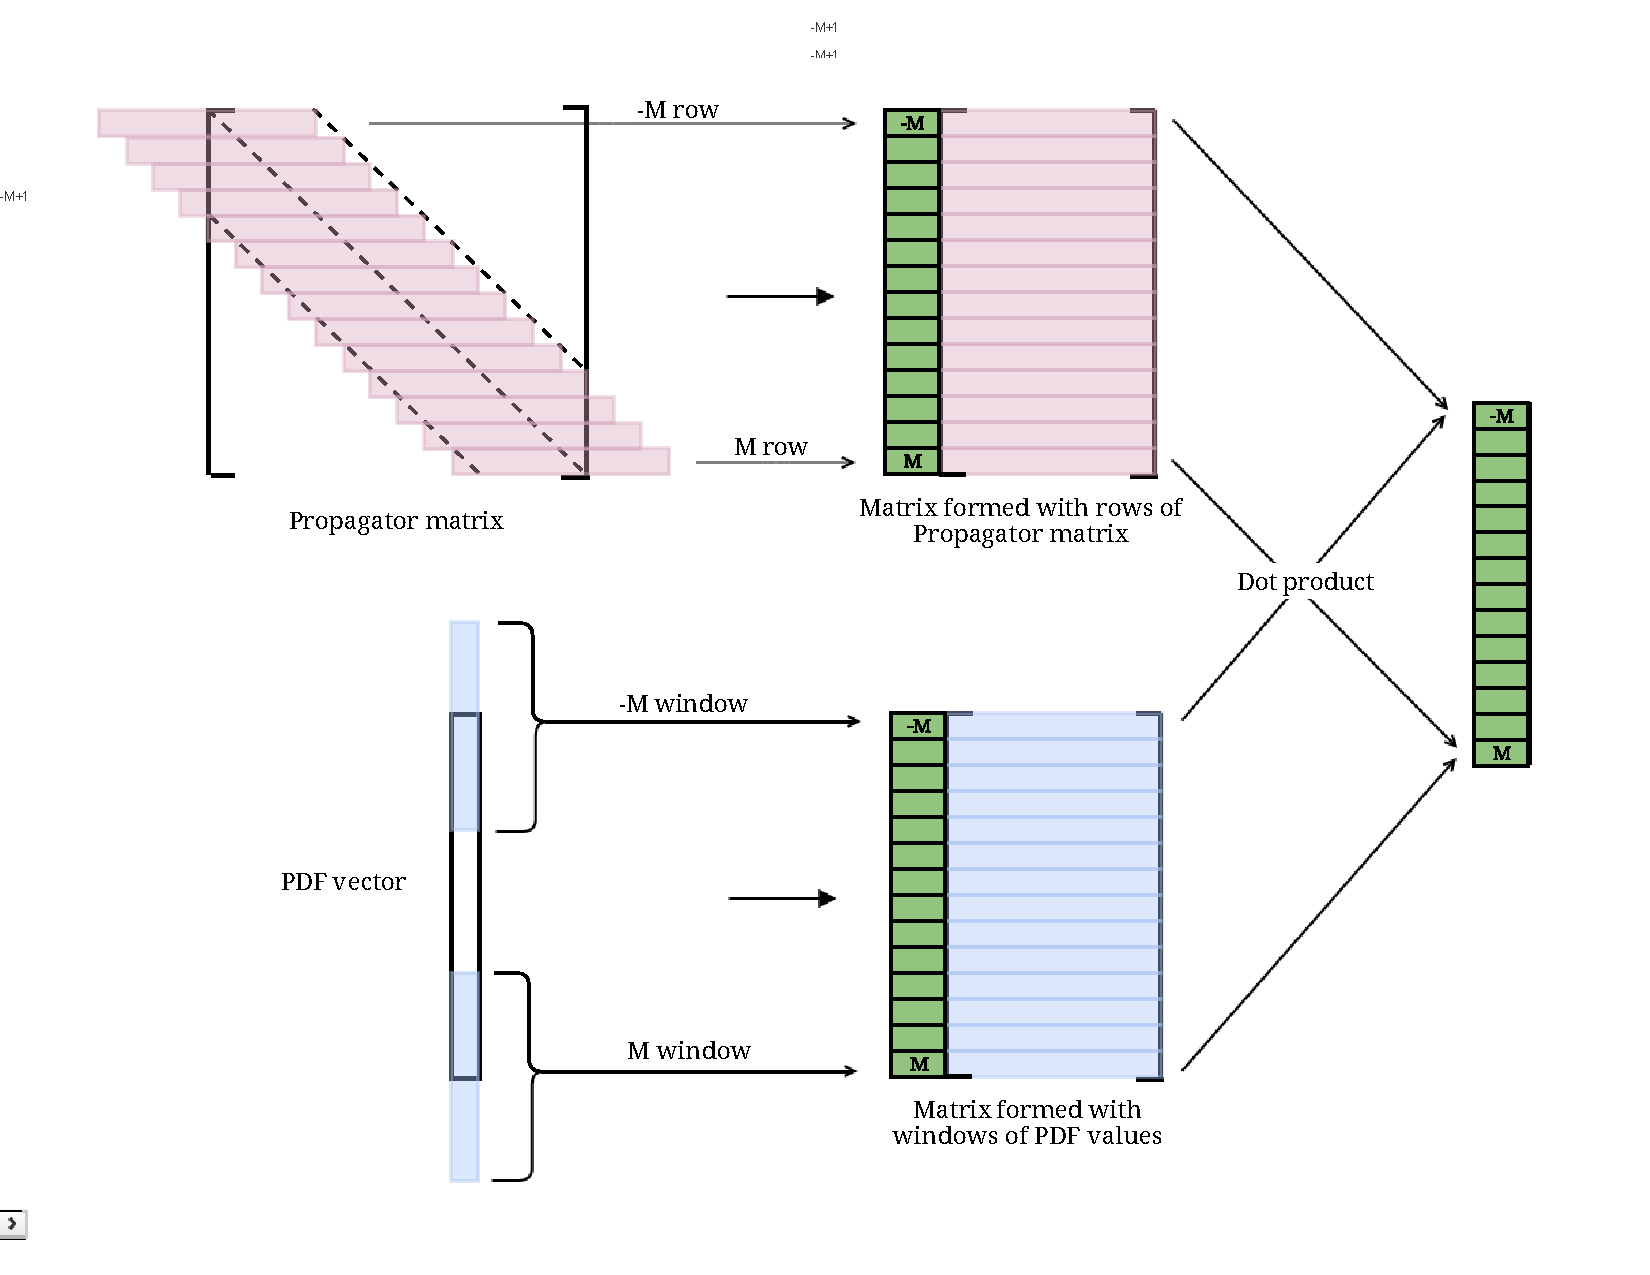
\includegraphics[width=6in]{gammawindow}
\end{center}
\caption{In order to implement the matrix-vector multiplication in
  (\ref{eqn:matrixchapman}) in a scalable way, we make use of the
  structure of the propagator matrix $\mathcal{G}$.  Instead of computing all
  entries of this matrix, we compute and store only those entries that
  are close to the diagonal---the pink rectangles in the upper half of
  the diagram.  The blue rectangles in the lower half of the diagram
  correspond to windowed versions of the pdf vector $\mathbf{p}_i$.
  In both cases, there is one windowed vector per row; the row numbers
  go from $-M$ to $M$ as labeled.  Both the pink and blue rectangles
  correspond to vectors of length  $2\gamma+1$, with $\gamma \ll M$.  The matrix-vector
  multiplication $\mathcal{G}  \mathbf{p}_i$ then corresponds to a
  collection of $2M+1$ vector-vector dot  products.  This
  representation of (\ref{eqn:matrixchapman}) makes efficient use of
  Scala, Breeze, and the Intel MKL.  For more details, see the description in Section \ref{sect:scala}.}
\label{fig:implementation1}
\end{figure}

\subsection{Spark}
\label{sect:spark}
Spark enables parallel/distributed computation using the notion of a
resilient distributed dataset (RDD).  Since the main bottleneck in our
Metropolis algorithm is the computation of the likelihood
$p(\mathbf{x} \, | \, \theta)$, we turn to the question of converting
the state time series $\mathbf{x}$ into an RDD.  We think of this time
series as a sequence of pairs $(t_j,x_j)$ as depicted in the
top line of Figure \ref{fig:implementation2}.  When we examine
(\ref{eqn:markov}), we see that to compute a given term in the product,
we need access to neighboring pairs $(t_j,x_j)$ and
$(t_{j+1},x_{j+1})$.

Hence, we map the original sequence of pairs,
labeled as $\overrightarrow{tx}$ in Figure \ref{fig:implementation2}, to
\texttt{tslices}, a Scala \texttt{Array} where each element is a
vector of neighboring pairs.  We convert this array to an RDD, \texttt{tslicesRDD}, using
Spark's \texttt{sc.parallelize} method.  When we subsequently use a
\texttt{map} operation to compute the log likelihood $\log p(x_{j+1} \, | \,
x_j, \theta)$ term corresponding to each element of \texttt{tslicesRDD},
the computation takes place in parallel.  Spark automatically
distributes the propagator and the $\theta$ vector.  For a
non-equispaced time series problem, each calculation of
$p(x_{j+1} \, | \, x_j, \theta)$ will take more (respectively, less)
time when $t_{j+1} - t_j$ is larger (respectively, smaller).  Again, Spark automatically
assigns tasks to workers to compute the overall log likelihood efficiently.

\begin{figure}[ht]
\begin{center}
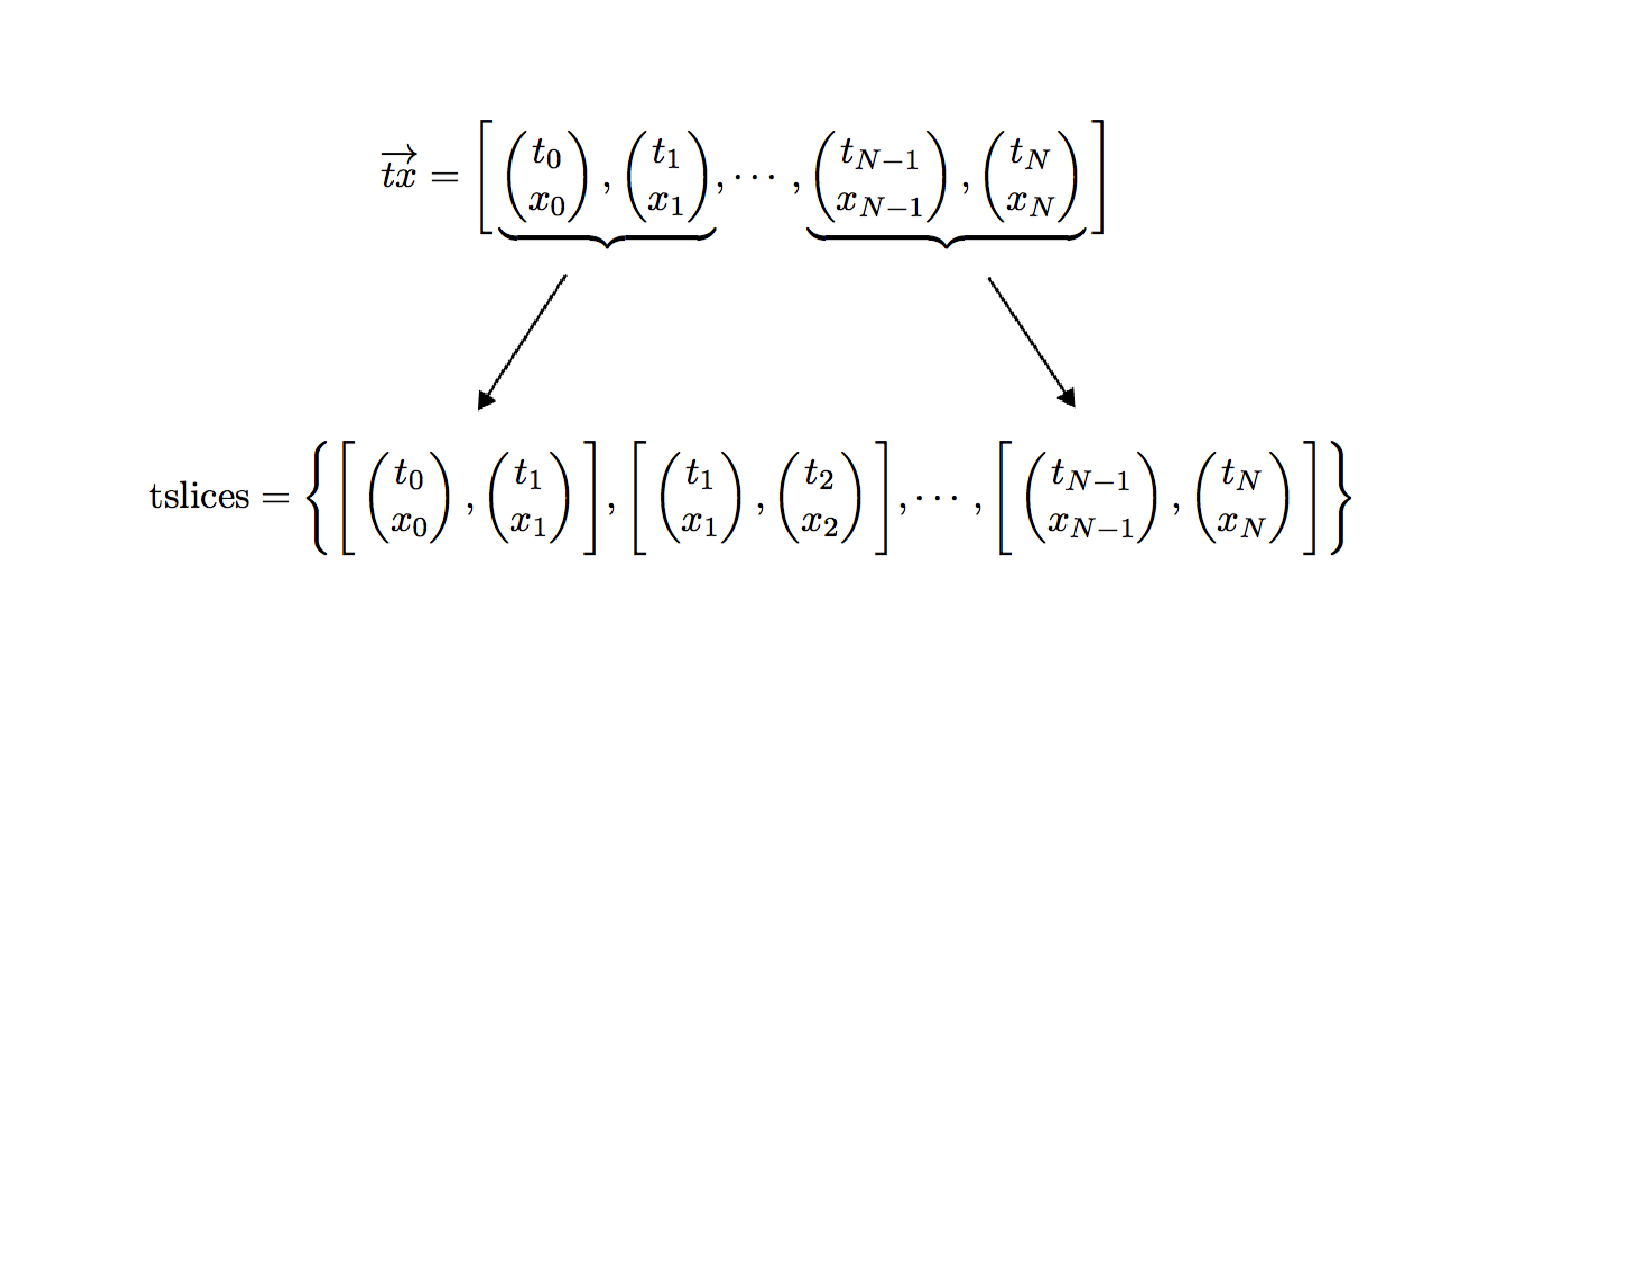
\includegraphics[width=6in]{vec_to_slice}
\end{center}
\caption{We use Spark to parallelize the computation of the likelihood
(\ref{eqn:markov}).  We accomplish this by converting the
original time series (for states $\mathbf{x}$, not observations
$\mathbf{y}$) from a vector of pairs to an array where each element is
a vector of consecutive pairs.  The original vector of pairs is
labeled as $\protect\overrightarrow{tx}$, and the Scala \texttt{Array}
of consecutive pairs is \texttt{tslices}.  This latter object can be
easily converted into a Spark RDD; subsequent \texttt{map} operations
on this RDD are executed in parallel.}
\label{fig:implementation2}
\end{figure}

\section{Results}
\label{sect:results}
We begin with results on artificial data sets.  The model used to
generate these data sets is the Ornstein-Uhlenbeck SDE
\begin{equation}
\label{eqn:ou}
{d}X_t = \theta_1 (\theta_2 - X_t) {d}t + \theta_3 {d}W_t
\end{equation}
together with the observation process
\begin{equation}
\label{eqn:ou_obs}
Y_t = X_t + \epsilon_t.
\end{equation}
Specifically, what we do is apply the Euler-Maruyama discretization to
(\ref{eqn:ou}) with a time step of $\kappa = 10^{-6}$.  Suppose our
temporal grid consists of $t_j = n(j) \kappa$, where $n(0) = 0$,
and $n(j+1) > n(j)$.  In some of the examples we pursue, $n(j)$ will
be deterministic and the temporal grid will be equispaced, while in other examples, $n(j)$ will
be stochastic and the temporal grid will be non-equispaced.  Either
way, we take $n(j)$ to have expected value $2 \times 10^5$, so that
the average difference between temporal grid points $t_{j+1} - t_j$ is $0.2$.

We then start at a
random initial condition by sampling $X_0$ from a Gaussian random
variable with mean $0$ and variance $1$.  We step forward one step at
a time (with time step $\kappa$), saving the numerical solution $X_t$
at points in time corresponding to the temporal grid points $\{t_j\}_{j=0}^L$.
We label the points we save as $(x_0, x_1, \ldots, x_L) =:
\mathbf{x}$, and then perturb them via (\ref{eqn:ou_obs}) to generate
$\mathbf{y}$.  In particular, we set $y_j = x_j + Z$ where $Z$ is
normally distributed with mean $0$ and variance $\sigma^2$.

The DTQ method described in Section \ref{sect:likelihood} has four
internal parameters: the time step $h$, the spatial grid spacing $k$,
the spatial grid cutoff $M$, and the decay width $\gamma$ of the Gaussian
kernel $G$.  For the tests described below, we will give the value of
$h$ that was used.  All other parameters are as follows: $k =
h^{0.75}$, $M = \lceil \pi/k^{1.5} \rceil$, and $\gamma = 25$.

\subsection{Equispaced Time Series}
\label{sect:equispaced}
In the first set of experiments, we follow the procedure outlined
above to generate artificial data $\mathbf{y}$ with the temporal grid
defined by $t_j = n(j) \kappa = (0.2) j$.  The ground truth for the
parameters consists of $\theta = (0.5, 1, 0.25)$ and $\sigma^2 =
0.01$.  In addition to the other parameters, we
focus on inferring $\theta_1$ and $\theta_2$; we fix $\theta_3 =
0.25$ throughout.  In the Metropolis algorithm, we take as initial conditions
$\mathbf{x}_0 = \mathbf{y}$, $\theta = (1,0.1,0.25)$, and
$\sigma_\epsilon^2 = 1$.

For priors for $\theta_1$ and $\theta_2$, we use Gaussian densities
with respective parameters $(\mu=0.5,\sigma=1)$ and
$(\mu=2,\sigma=10)$.  For $\sigma_\epsilon^2$, we use an exponential
prior with parameter $\lambda=1$.

In the Metropolis algorithm, we take all proposal random variables to
be independent Gaussians.  In particular, $Z_\mathbf{x}$ is a collection of
$L+1$ independent Gaussians, each with parameters
$(\mu=0,\sigma=0.02)$, $Z_\theta$ consists of two independent
Gaussians, each with parameters $(\mu=0,\sigma=0.05)$, and $Z_\sigma$
consists of a Gaussian with parameters $(\mu=0,\sigma=0.02)$.  These
distributions have been chosen, via trial and error, to yield a
Metropolis acceptance rate that is between $20-40\%$ in all tests we
have conducted.

For two values of the DTQ internal time step ($h = 0.02$ and
$h=0.01$), we apply the Metropolis algorithm to generate $10,000$
samples of the posterior (\ref{eqn:post2}).  Note that $h=0.02$
implies $M=257$ and $h=0.01$ implies $M=559$; hence $\gamma=25$
gives at least a $10$-fold reduction in computational effort.

We discard the first $100$ samples as burn-in samples, i.e., samples
that are taken before the Metropolis Markov chain has, to a good
approximation, reached equilibrium.

Using the samples thus obtained, we plot the posterior densities for
$\theta_1$, $\theta_2$ and $\log_{10} \sigma_\epsilon^2$ in Figure
\ref{fig:post_equi}.  In this paper, all density plots use a Gaussian
kernel with the ``nrd'' (or normal reference rule) bandwidth
\citep{Scott2015}.  The density in blue (respectively, black)
corresponds to the samples produced using the DTQ method with $h=0.02$
(respectively, $h=0.01$).  The red vertical lines indicate the ground
truth values for each parameter.

Overall, we see that the Metropolis algorithm does a reasonable job of
inferring the parameters.  For the Orstein-Uhlenbeck model
(\ref{eqn:ou}), Bayesian inference is non-trivial when the temporal
spacing between observations is sufficiently large.  Keeping in mind
the logarithmic scale for the density of the third parameter, we still
conclude that our method has the greatest room for improvement here.
As we show below, however, the mean inferred value of
$\sigma_\epsilon$ is consistent with the observation series
$\mathbf{y}$ and the mean inferred state series $\mathbf{x}$.

\begin{figure}[th]
\begin{center}
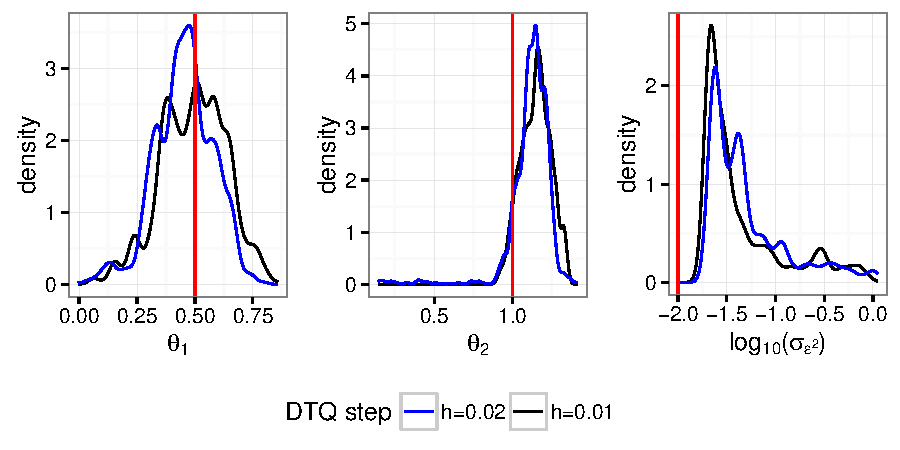
\includegraphics[width=6in]{post_equi}
\end{center}
\caption{Posterior densities for the inference/filtering problem with
  equispaced time series $(\mathbf{t},\mathbf{y})$.  Each density is
  calculated on the basis of $9900$ post-burn-in Metropolis samples
  computed  using the indicated value of the internal DTQ time step
  parameter $h$.  Overall, we see reasonable agreement between the
  ground truth values (indicated by red vertical lines) and the
  posterior densities.}
\label{fig:post_equi}
\end{figure}

\subsection{Non-equispaced Time Series}
\label{sect:nonequispaced}
In this next set of experiments, we follow a nearly identical
procedure to that described in Section \ref{sect:equispaced}.  The
main difference is that the temporal grid is defined by $t_j = n(j)
\kappa$ where $n(j)$ is uniformly distributed on the integers between
$4 \times 10^{4}$ and $4 \times 10^5 - 4 \times 10^4$.  Effectively,
this generates a time series with minimum, mean, and maximum spacings
$t_{j+1} - t_j$ of, respectively, $0.04$, $0.2$, and $0.36$.

We use the same priors and Metropolis initial conditions as in Section \ref{sect:equispaced}.  We change
the proposal distributions slightly.  The parameters for
$Z_{\mathbf{x}}$ and $Z_\sigma$ are now $(\mu=0,\sigma=0.01)$, while
for $Z_\theta$ the parameters are still $(\mu=0,\sigma=0.05)$.

For two values of the DTQ internal time step ($h = 0.02$ and
$h=0.01$), we apply the Metropolis algorithm to generate $10,000$
samples of the posterior (\ref{eqn:post2}).  Again, we discard the
first $100$ samples as burn-in samples.

Using the samples thus obtained, and using the same procedure
described in Section \ref{sect:equispaced}, we plot the posterior densities for
$\theta_1$, $\theta_2$ and $\log_{10} \sigma_\epsilon^2$ in Figure
\ref{fig:post_nonequi}.  Overall, as compared with Figure
\ref{fig:post_equi}, we see improved agreement between the ground
truth values and the posteriors for $\theta_2$ and
$\log_{10}$, while the posterior for $\theta_1$ is still reasonably
accurate.


\begin{figure}[th]
\begin{center}
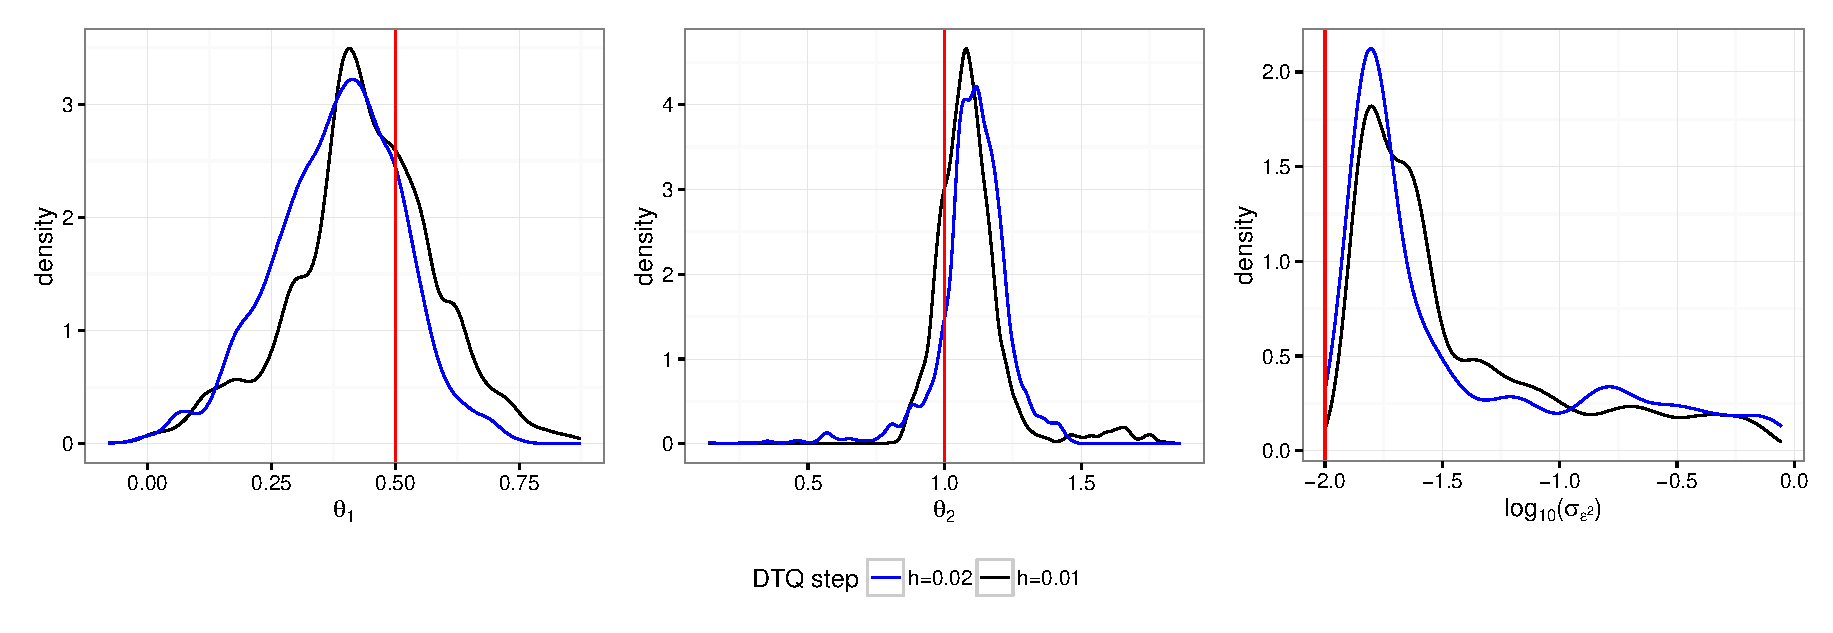
\includegraphics[width=6in]{post_nonequi}
\end{center}
\caption{Posterior densities for the inference/filtering problem with
  non-equispaced time series $(\mathbf{t},\mathbf{y})$.  Each density is
  calculated on the basis of $9900$ post-burn-in Metropolis samples
  computed  using the indicated value of the internal DTQ time step
  parameter $h$.  Overall, we see reasonable agreement between the
  ground truth values (indicated by red vertical lines) and the
  posterior densities.}
\label{fig:post_nonequi}
\end{figure}


We turn to the filtering results, focusing on the post-burn-in samples of
$\mathbf{x}$ generated with DTQ parameter $h=0.01$.  In Figure
\ref{fig:timeseries1}, we plot the original non-equispaced observation
series $\mathbf{y}$ in red.  We have plotted in grey each of the
$9900$ samples of the state series $\mathbf{x}$; the mean of these
samples is plotted in black.  We see that the Metropolis sampler does
indeed explore a number of different trajectories for the state
series, and that the mean inferred state series corresponds to a
smoothed version of the original observation series.


\begin{figure}[th]
\begin{center}
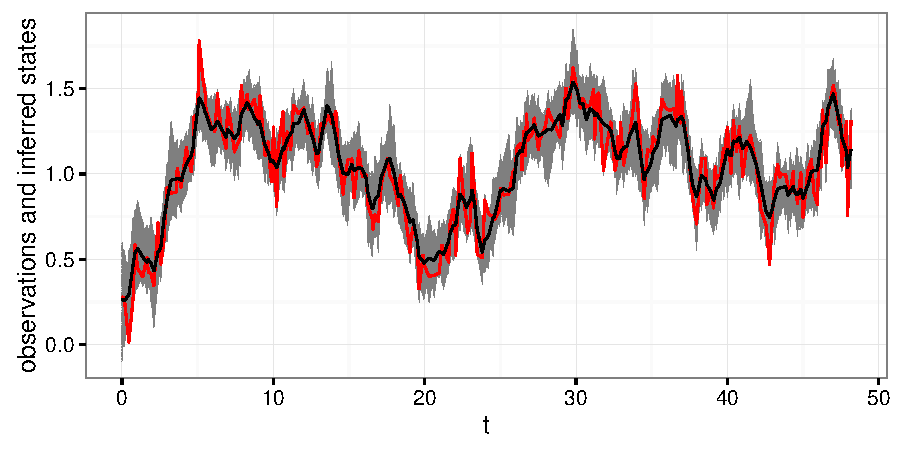
\includegraphics[width=6in]{timeseries1}
\end{center}
\caption{We plot the observations (in red) together with each of the
  samples of the state series $\mathbf{x}$.  Each such sample is a
  grey curve, and the mean of all such grey curves is plotted in
  black.  We refer to the black curve as the mean inferred state series.}
\label{fig:timeseries1}
\end{figure}


In Figure \ref{fig:timeseries2}, we again plot the original
non-equispaced observation series $\mathbf{y}$ in red and the mean
inferred state series $\mathbf{x}$ in black.  This time,
however, we add/subtract the mean inferred value of $\sigma_\epsilon$
to $\mathbf{y}$ to obtain error bars associated with each
observation.  These error bars are plotted in grey.  The idea behind
this plot is that if (\ref{eqn:obs}) holds, then given the symmetry of
the random variables $\epsilon_t$, it should also be true that $X_t =
Y_t + \epsilon'_t$, where $\epsilon'_t$ has the same distribution as
$\epsilon_t$.  To be self-consistent, the observation series should,
at least most of the time, lie within one (inferred) standard deviation
$\sigma_\epsilon$ of the (inferred) state series.  The plot in Figure
\ref{fig:timeseries2} confirms that this is the case.

\begin{figure}[th]
\begin{center}
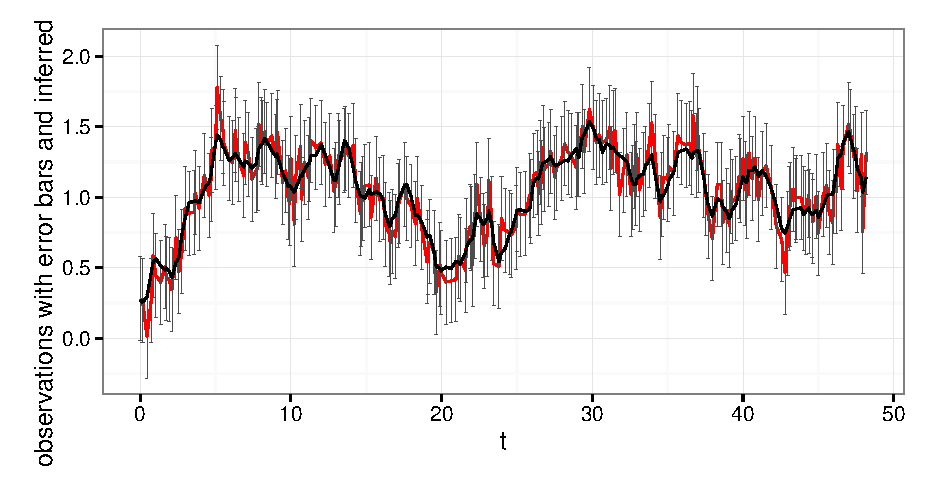
\includegraphics[width=6in]{timeseries2}
\end{center}
\caption{We plot the observations (in red) together with the mean
  inferred state series (in black).  The
  error bars (grey) are computed by adding/subtracting the mean inferred
  value of $\sigma_\epsilon$ to/from the observation series
  $\mathbf{y}$.  Note that the mean inferred state is typically within
one $\sigma_\epsilon$ of the corresponding observation.}
\label{fig:timeseries2}
\end{figure}

\subsection{Scaling}
\label{sect:scaling}
We have conducted tests to explore the relationship between running
time and $L$, the length
of the observation series.  For each $L \in \{124, 250, 500,
2500\}$, and for each $h \in \{0.02, 0.01\}$, we have generated a
time series of the indicated length, run our inference/filtering code, and
recorded the amount of time $T$ required to generate $1000$ Metropolis
samples of the posterior.  The results are plotted in Figure
\ref{fig:scaling} with log-transformed axes. For each set of points,
we fit a line of the form $\log T = \beta_0 + \beta_1 \log L$, which
corresponds to the law $T = e^{\beta_0} L^{\beta_1}$.  The solid lines
in Figure \ref{fig:scaling} correspond to this latter law, plotted on
the same log-transformed axes.  For the $h=0.02$ line, we obtain
$\beta_1 = 0.9092$; for the $h=0.01$ line, we obtain
$\beta_1=0.9639$.  These results are consistent with $O(L)$ temporal scaling.

\begin{figure}[th]
\begin{center}
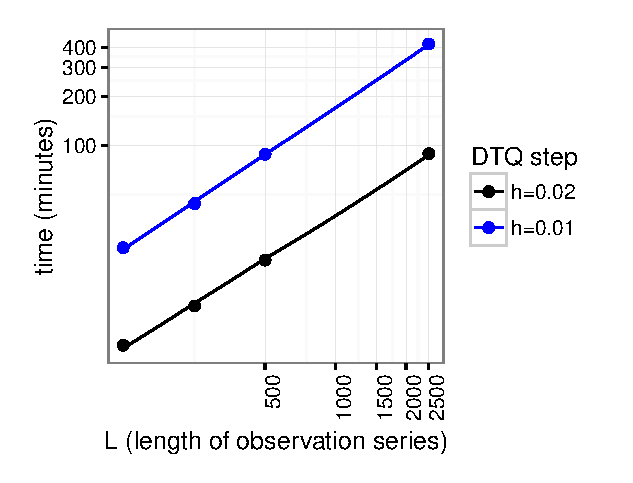
\includegraphics[width=5in]{scaling}
\end{center}
\caption{For each indicated value of $L$, we have generated a time
  series of length $L$, run our inference/filtering code, and recorded
  the amount of time $T$ required to generate $1000$ Metropolis samples of
  the posterior.  We fit lines to $\log T$ as a function of $\log
  L$---both the lines and the original data are plotted on
  log-transformed axes.  The slopes of the lines are less than $1$,
  consistent with $O(L)$ temporal scaling.}
\label{fig:scaling}
\end{figure}


\section{Discussion and Conclusion}
\label{sect:conclusion}
The results from Section \ref{sect:results}
show that while decreasing the value of the DTQ internal step $h$ does
change the sampled values and the plotted densities, the change is not
significant.  We believe much greater gains (in terms of agreement
between the posterior modes and the ground truth values) would be achieved by
improving both the proposal strategy and the vanilla Metropolis
accept/reject step; such ideas have been pursued successfully by \citep{Fuchs2013} and others, and we seek
to implement these improvements in future work.  For now, however, we
conclude that the implementation described in this paper does indeed
perform Bayesian filtering and inference at a baseline acceptable
level.

Aside from improving the Metropolis algorithm, we see three main
areas for improvement.  First, we have yet to test and tune our implementation
on a large-scale, distributed Spark cluster. 
Second, we believe we can derive large gains in performance by
adapting our algorithm to work in a streaming fashion.  Specifically,
instead of inferring the entire state series $\mathbf{x}$ at once, as
we currently do, we can proceed one step a time through the temporal
sequence of observations.  Third, we have already begun to incorporate
the DTQ into an adjoint method suitable for computing gradients of the
likelihood.  This will enable us to apply techniques such as
stochastic gradient descent or Hamiltonian Monte Carlo to our
inference problem for either fast MLE/MAP point estimation or
accelerated sampling from posteriors.  These steps, and possibly
others, will become  necessary as we adapt our methods to
multi-dimensional time series problems, a task we have already begun.

\acks{This work was partially supported by a grant from UC Merced's
  Committee on Research (awarded to H.S. Bhat) and by UC Merced USAP fellowships
  (awarded to R.W.M.A. Madushani and S. Rawat).}

\bibliography{BhatMaduRawatBigMine16}

\end{document}

%%% Local Variables:
%%% mode: latex
%%% TeX-master: t
%%% End:
